\documentclass{article}
\usepackage[x11names, rgb]{xcolor}
\usepackage[utf8]{inputenc}
\usepackage{tikz}
\usetikzlibrary{snakes,arrows,shapes}
\usepackage{amsmath}
% from http://www.fauskes.net/code/dot2tex/gallery/tikz-node-shapes/
%
%
%

\begin{document}
\pagestyle{empty}
%
%
%

\enlargethispage{100cm}
% Start of code
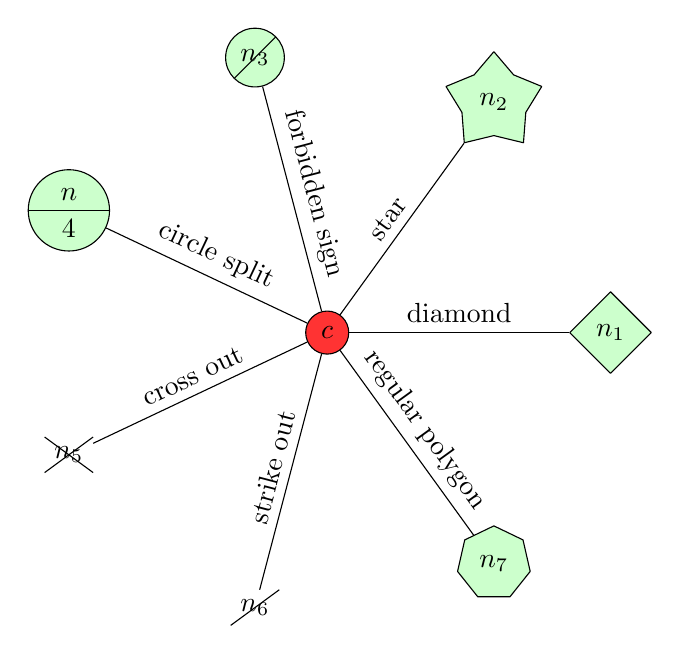
\begin{tikzpicture}[>=latex',join=bevel,]
%
\node (c) at (121bp,118bp) [draw,circle,fill=red!80] {$c$};
  \node (n_1) at (223bp,118bp) [draw,diamond,fill=green!20] {$n_1$};
  \node (n_2) at (181bp,201bp) [draw,star,fill=green!20] {$n_2$};
  \node (n_3) at (95bp,217bp) [draw,forbidden sign,fill=green!20] {$n_3$};
  \node (n_4) at (28bp,162bp) [draw,circle split,fill=green!20] {$n$ \nodepart{lower} $4$};
  \node (n_5) at (28bp,74bp) [draw,cross out,fill=green!20] {$n_5$};
  \node (n_6) at (95bp,19bp) [draw,strike out,fill=green!20] {$n_6$};
  \node (n_7) at (181bp,35bp) [draw,regular polygon,regular polygon sides=7,fill=green!20] {$n_7$};
  \draw [] (c) -- node[above,sloped] {diamond} (n_1);
  \draw [] (c) -- node[above,sloped] {star} (n_2);
  \draw [] (c) -- node[above,sloped] {forbidden sign} (n_3);
  \draw [] (c) -- node[above,sloped] {circle split} (n_4);
  \draw [] (c) -- node[above,sloped] {cross out} (n_5);
  \draw [] (c) -- node[above,sloped] {strike out} (n_6);
  \draw [] (c) -- node[above,sloped] {regular polygon} (n_7);
%
\end{tikzpicture}
% End of code

%
\end{document}
%


